\documentclass[a4paper,12pt]{article}
\usepackage{czech}
\usepackage[utf8]{inputenc}
\usepackage{a4wide}
\usepackage[dvipdfm]{graphicx}
\usepackage{graphics}
\usepackage{indentfirst}
\usepackage{fancyhdr}
\usepackage{setspace}
\usepackage{amsmath}
\usepackage{amssymb}
\usepackage{epsfig}

%%\usepackage{nopageno}
%%\usepackage{txfonts}
\usepackage[usenames]{color}
\renewcommand{\d}{\mbox{d}}

\begin{document}
\section{Úkol}
\begin{enumerate}
\item Změřte střední velikost zrna připraveného vvýbrusu polykrystalického vzorku. K vyhodnocení snímku ze skenovacího elektronového mikroskopu použijte kruhovou metodu.
\item Určete frakční objem dendritických částic v eutektické slitině Mg-Al-Ce. Použijte specializované programové vybavení pro obrazovou analýzu.
\end{enumerate}

\section{Úvod}
Elektronový mikroskop má řadu požných  použití napříč vědnímy obory. Jeho rozlišovací schopnost je pohybuje v řádu nanometrů, což je hojně používáno ke zkoumání povrchů. Transmisní elektronové miskroskopy se následně užívají ke zkoumání vnitřích struktur materiálu. Jak bylo naznačeno ve fyzivce se používá především k analýze materiálů, pozorování jejich struktur a určování vad.

\section{Měření}
\subsection{Fe$_3$Al}
Nejprve jsme se zabývali chování Fe$_3$Al v závislosti na teplotě. Tento materiál se totiž za pokojových teplo jeví pevný a křehký. Pokud 
ho však zahřejeme na teplotu okolo 700 $^\circ$C, materiál se stane tvárným. 

Na obrázku (\ref{o1}) můžeme vidět snímek z elektronového mikroskopu za pokojevé teploty. Materiál je zjevně tvořen zrny, jjichž hranice 
jsou slabinou ve struktuře, po které může postupovat porucha. Tak dochází ke křehkému interkristalickému lomu a proto materiál není tvárný. 

Naproti tomu při pohledu na obrázek (\ref{o2}), který je pořízen za teploty okolo 700 $^\circ$C vidíme, že zrnovitá stuktura byla nahrazena 
zcela jinou, která již plastckou deformaci umožňuje.

\subsection{Velikost zrna}
Dále jsme zkoumali velikost zrna materiálu na obrázku (\ref{o3}), na kterém jsou zjevné důsledky koroze. Předpokládámě, že materiál je homogení a izotropní. Díky 
tomu můžeme zrna aproximovat koulemi a použít vzorec 
\begin{eqnarray}
d=\frac{3\pi}{2}\frac{D}{n},
\end{eqnarray}
kde $D$ je průměr kružnice a $n$ počet protnutých zrn kružnicí. Na obrázku můžeme vidět 5 kružnic o poloměrech
\begin{eqnarray}
r_1=0.0462\ \mbox{mm} \\
r_2=0.0423\ \mbox{mm} \\
r_3=0.0407\ \mbox{mm} \\
r_4=0.0435\ \mbox{mm} \\
r_5=0.0468\ \mbox{mm}
\end{eqnarray}
Velikosti zrn určená z jednotlivých kružnic jsou
\begin{eqnarray}
d_1=(0.009 \pm 0.001)\ \mbox{mm} \\
d_2=(0.009 \pm 0.001)\  \mbox{mm} \\
d_3=(0.008 \pm 0.001)\  \mbox{mm} \\
d_4=(0.008 \pm 0.001)\ \mbox{mm} \\
d_5=(0.009 \pm 0.001)\  \mbox{mm} 
\end{eqnarray}
což nám dá po statistickém vyhodnocení
\begin{eqnarray}
d=(0.0086 \pm 0.0004)\ \mbox{mm}
\end{eqnarray}
V chybě je zahrnuta nejistota způsobená nejednoznačností  zrn mající společnou hranici s kružniví a neurčitost chybějících zrn vniklých korozí.

\subsection{MgAlCe}
Pro dobré určení frakčního objemu dendrických částí ve sloučeníně bychom potřebovali aspoň pět snímků. K dispozici však máme pouze jeden, proto je celé měření zatíženo velkou chybou. Dále jse binarizace obrazu značně subjektivní 
metoda. Jako poslední jemná chyba se projevila nepřesnost v určení rozměru "čtvercového" obrazu, kde došlo k chybě 0.0005 mm. O vzorku jsme dále předpokládali, že je homogení a izotropní. Výsledná chyba je odhadnuta na 20 procent. Dle použitého programu byl obsha dendricých částic 
\begin{eqnarray}
S=998.9082\ \mu\mbox{m}^2
\end{eqnarray}
Po započtení chyb tedy dostáváme poměr dendrických částic ku celku
\begin{eqnarray}
P=0.16\pm0.03
\end{eqnarray}
Nakonec jsem pomocí programu vytvořil hystogram zastoupení shluků podle velikosti. Výsledky jsou v tabulce \ref{his}

\begin{table}
$$
\begin{array}{|c|c|c|c|}
\hline
\mbox{počet č.}&    S/\mu\mbox{m}^2& P& \mbox{průměrná vel.}/\mu\mbox{m}^2 \\ \hline
153&    822.46& 0.823&  5.37 \\ \hline
2&  70.98&  0.071&  35.5 \\ \hline
1&  105.5&  0.106&  105.5 \\ \hline
\end{array}
$$
\caption{Histogram zastoupení dendrických částic dle velikosti shluků.}
\label{his}
\end{table}

\section{Diskuze}
Užité metody a zařízení jsou dobré ke kvalitativní analýze problému a seznámení s použitím elektronového mikroskopu. Pokud bychom však chtěli data s použitelnou chybou, muselo by proběhnou výrazně více měření na více vzorcích, předevěím 
pro to, abychom ověřili homogenitu a izotropii zkoumaných materiálů. Subjektivní faktor by však omezila pouze změna metody.

\section{Závěr}
l jsem velikost zrna vzorku, která byla
\begin{eqnarray}
d=(0.0086 \pm 0.0004) \mbox{mm}
\end{eqnarray}
Určil jsem frakční objem dendrických částic ve slitině MgAlCe
\begin{eqnarray}
P=0.16\pm0.03
\end{eqnarray}

\begin{figure}[!htb]
\begin{center}
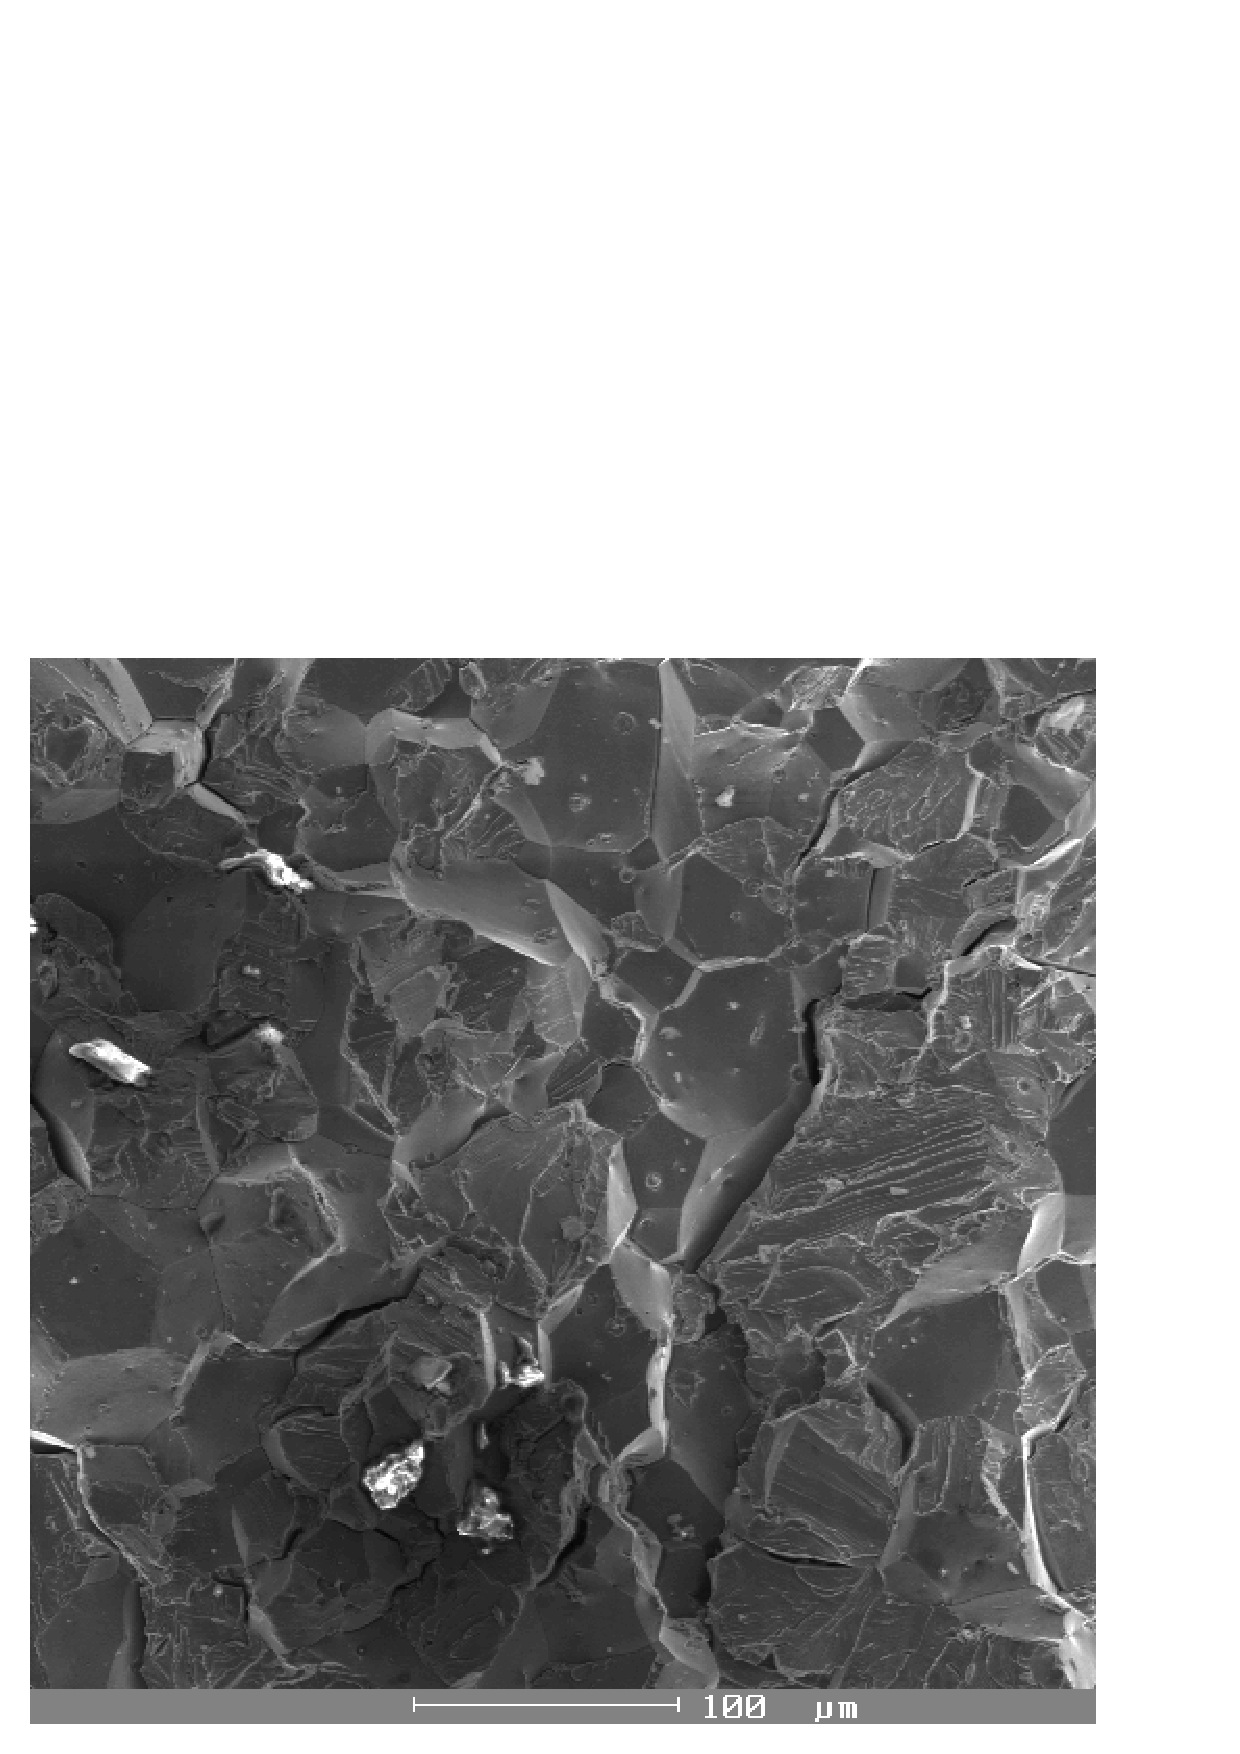
\includegraphics[scale=.7]{B1.png}
\end{center}
\caption{Snímek Fe$_3$Al za pokojové teploty}
\label{o1}
\end{figure}

\begin{figure}[!htb]
\begin{center}
\includegraphics[scale=.7]{B2.png}
\end{center}
\caption{Snímek Fe$_3$Al za teploty 700 $^\circ$C}
\label{o2}
\end{figure}

\begin{figure}[!htb]
\begin{center}
\includegraphics[scale=.7]{B3.png}
\end{center}
\caption{Snímek výbrusu.}
\label{o3}
\end{figure}

\begin{figure}[!htb]
\begin{center}
\includegraphics[scale=.7]{B4.png}
\end{center}
\caption{Snímek slitiny MgAlCe}
\label{o4}
\end{figure}

\begin{figure}[!htb]
\begin{center}
\includegraphics[scale=.7]{B5.png}
\end{center}
\caption{Binarizovaný snímek slitiny MgAlCe}
\label{o5}
\end{figure}

\begin{thebibliography}{5}
	\bibitem{text} \textbf{Studijní text na praktikum IV} \\http://physics.mff.cuni.cz/vyuka/zfp/txt\_418.pdf (17. 12. 2012)
\end{thebibliography}


\end{document}
